
\chapter{Governing equations for free surface flows}
\label{equations}


In this chapter a bibliographic revision of the methods employed to solve free surface flows problems is presented.
The analysis of the numerical methods for the shallow water equations is more extensive than the review for the Navier-Stokes equations, since this thesis presents some advances in the numerical simulation of the shallow water equations.
Before introducing the review of the numerical methods, the governing equations will be presented.
The following sections are devoted for the numerical methods.
The last section is about the coupling algorithms.



%\section{Free surface flows}


Among the water related phenomena, natural hazards usually involve free surface flows.
This property allow to assume some simplifications, specially at the large scale.
For this reason, the Navier-Stokes equations are briefly presented before introducing the depth integrated models.



\section{Navier-Stokes equations}


The motion of a fluid is described by the Navier-Stokes equations. The case of a free surface flow is described by that equations and the free surface is located where the densities or the fluid properties are discontinuous. In general, an air-water interface is assumed but some natural phenomena may include a more complex configuration, such as debris flow-air-water interfaces. All this continuous media can be considered isotermal and incompressible, and the standard formulation of the Navier-Stokes equations can be used.

The problem consists in the incompressible Navier-Stokes equations in a time interval $(0, t_f)$ and in a spatial domain $\Omega \in \mathbb{R}^{n_d}$, being $n_d$ the number of space dimensions, $3$ unless otherwise stated. Let $t$ be a certain time instant in the temporal domain $(0, t_f)$ and $\mathbf{x}$ a given point in the spatial domain $\Omega$. The balance equations for the momentum and mass are written in the following form:
\begin{subequations}
    \begin{align}
        \pder{u_i}{t} + u_j \pder{u_i}{x_i} + \frac{1}{\rho} \pder{p}{x_i} +
            \frac{1}{\rho} \pder{}{x_i} \tau_{ij} &= f_i \\
        \pder{u_i}{x_i} &= 0
    \end{align}
\end{subequations}
With the appropriate initial and boundary conditions. Let $\Gamma$ be the boundary of the domain $\Omega$ and $\mathbf{n}$ the unit outward normal on $\Gamma$. Dirichlet and Neumman boundary conditions are considered, $\Gamma_D$ and $\Gamma_N$ respectively, such that $\Gamma_D \cup \Gamma_N = \Gamma$.
The usual summation convention is used if there is index repetition.
$\rho$ is the fluid density, $p$ is the pressure, $\mathbf{u}$ is the velocity, $\bm{\tau}$ is the viscous stresses tensor and $\mathbf{f}$ is the body forces vector.



\subsection{Shallow water equations}



The shallow water equations are the result of integrating vertically the Navier-Stokes equations, assuming the vertical velocity and its acceleration negligible \cite{abbot1979,zien3}.
The equations governing mass and momentum conservation can be written in conservative form with water depth $h$ and specific discharge $\mathbf{q}=(h\mathbf{u})$ as follows,

\begin{equation} \label{general_sw}
\pder{\bm{\phi}}{t} + \pder{\mathbf{F}_i}{x_i} + \pder{\mathbf{G}_i}{x_i} + \mathbf{Q} = \mathbf{0} \quad \text{for} \enspace i=1,2
\end{equation}
with

\begin{subequations}\label{variables_and_fluxes}
\allowdisplaybreaks
\begin{align}
\bm{\phi} &= \left\{
    \begin{array}{c}
        hu_1 \\
        hu_2 \\
        h
    \end{array}\right\} \\
\mathbf{F}_i &= \left\{
    \begin{array}{c}
        hu_1u_i + \delta_{1i}\frac{1}{2}g(h^2 - z^2) \\ [5pt]
        hu_2u_i + \delta_{2i}\frac{1}{2}g(h^2 - z^2) \\ [5pt]
        hu_i
    \end{array}\right\} \\
\mathbf{G}_i &= \left\{
    \begin{array}{c}
        -(h/\rho) \bar{\tau}_{1i} \\ [5pt]
        -(h/\rho) \bar{\tau}_{2i} \\ [5pt]
        0
    \end{array}\right\} \\
\mathbf{Q} &= \left\{
    \begin{array}{c}
        \displaystyle -g(h-z)\pder{z}{x_1} + \frac{h}{\rho}\pder{p_a}{x_1}
        - \frac{1}{\rho}\tau^s_{31} + \frac{1}{\rho}\tau^b_{31} \\ [10pt]
        \displaystyle -g(h-z)\pder{z}{x_2} + \frac{h}{\rho}\pder{p_a}{x_2}
        - \frac{1}{\rho}\tau^s_{32} + \frac{1}{\rho}\tau^b_{32} \\ [10pt]
        r
    \end{array}\right\}
\end{align}
\end{subequations}
where $\bm{\phi}$ is the vector of conserved variables, $\mathbf{F}_i$ is the vector of convective fluxes, $\mathbf{G}_i$ is the vector of viscous fluxes and $\mathbf{Q}$ is the vector source terms. In Figure \ref{diagram} there is a representation of the variables and the notation. The coordinates are denoted with the index notation $x_i$. Since this formulation is defined in a two dimensional space ($n_d=2$), in the following we will consider $i=1,2$.
$\delta_{ij}$ is the Kronecker delta. The topography is expressed with the variable $z$ and the free surface elevation is expressed in terms of the topography and the total depth, $\eta = z + h$. $\bar{\tau}_{ij}$ are the averaged horizontal stresses, and $\tau^b_{3i}$ and $\tau^s_{3i}$ denote the bottom and surface friction stresses respectively. Finally, $r$ is the rain source term and $p_a$ is the atmospheric pressure.


\begin{figure}
    \centering
    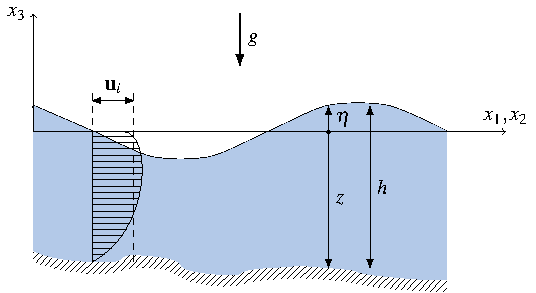
\includegraphics[width=.8\textwidth]{img/diagram.pdf}
    \caption{Diagram and notation for the balance equations (\ref{general_sw}) and (\ref{variables_and_fluxes})}
    \label{diagram}
\end{figure}

The problem is closed with an initial boundary condition,

\begin{equation}
\bm{\phi}(t=t_0) = \bm{\phi}_0
\end{equation}
where $\bm{\phi}_0$ are the initial water height and specific discharge.


The following Dirichlet boundary conditions are considered covering all the boundary $\Gamma$ of the domain $\Omega$:
\begin{itemize}
    \item Inflow boundary: the flow rate is known
    \begin{equation*}
        \mathbf{q} = \mathbf{q}_{in} \quad \text{in} \quad \Gamma_{in}
    \end{equation*}
    If the inflow is supercritical, the water depth is also specified
    \begin{equation*}
        \left.\begin{matrix}
        \mathbf{q} = \mathbf{q}_{in} \\
        h = h_{in}
        \end{matrix}\right\}
        \quad \text{in} \quad \Gamma_{in}
    \end{equation*}
    \item Outflow boundary: the water depth is known
    \begin{equation*}
        h = h_{out} \quad \text{in} \quad \Gamma_{out}
    \end{equation*}
    if the outflow is supercritical, no conditions have to be imposed.
    \item Solid boundary: slip or no slip condition can be imposed
    \begin{equation*}
        \mathbf{q} \cdot \mathbf{n} = 0 \quad \text{or} \quad \mathbf{q} = \mathbf{0} \quad \text{in} \quad \Gamma_{solid}
    \end{equation*}
\end{itemize}


The bottom friction $\tau^b_{3i}$ is modelled with the Manning formula generalized for two dimensions as

\begin{equation}
\frac{\tau^b_{3i}}{\rho} = -gn^2\frac{\abs{\mathbf{q}}\mathbf{q}}{h^{\sfrac{7}{3}}}
\end{equation}
where $n$ is the Manning coefficient. It defines the resistance to flow by the roughness of the bottom or other macroscopic factors and it is determined empirically. In practice, the Manning coefficient varies from 0.01 for a very smooth bed (concrete) to 0.05 for a rough bed (rocks) \cite{chow1988}.


The averaged horizontal stresses are calculated from the combination of the molecular stresses and the Reynolds stresses as follows
\begin{equation} \label{stresses}
\frac{\bar{\tau}_{ij}}{\rho} = (\nu + \nu_t)\left(
    \pder{u_i}{x_j} + \pder{u_j}{x_i} -\frac{2}{3}\delta_{ij}\pder{u_k}{x_k} \right)
\end{equation}
where $\nu$ is the kinematic viscosity and $\nu_t$ is the turbulent kinematic viscosity. When any model of turbulence is considered, the turbulent stresses can be included in the bottom friction with the Manning formula \cite{blade2005}. In this work, the turbulent stresses will be neglected.

The balance equation (\ref{general_sw}) is linearized in the following form

\begin{equation}
\pder{\bm{\phi}}{t} + \mathbf{A}_i\pder{\bm{\phi}}{x_i}
 - \pder{}{x_{i}}\left(\mathbf{K}_{ij}\pder{\bm{\phi}}{x_j}\right) + \mathbf{S}\bm{\phi} + \mathbf{b}_i\pder{z}{x_i} = 0
\end{equation}
where the matrices $\mathbf{A}_i$ and $\mathbf{K}_{ij}$ are the linearization matrices of the convective fluxes and the diffusive fluxes respectively. The convective matrices $\mathbf{A}_i$ are obtained after applying the chain rule to the vector of fluxes $\mathbf{F}_i$,
\begin{subequations}
\begin{align}
\pder{\mathbf{F}_i}{x_i} &= \pder{\mathbf{F}_i}{\bm{\phi}}\pder{\bm{\phi}}{x_i} \\
\mathbf{A}_i &= \pder{\mathbf{F}_i}{\bm{\phi}}
\end{align}
\begin{equation}
\mathbf{A}_1 = \left[\begin{matrix}
        2u_1 & 0   & -u_1^2 + c^2 \\
        u_2  & u_1 & -u_1 u_2 \\
        1    & 0   & 0
    \end{matrix} \right]
\quad , \quad
\mathbf{A}_2 = \left[\begin{matrix}
        u_2 & u_1  & -u_1 u_2 \\
        0   & 2u_2 & -u_2^2 + c^2 \\
        0   & 1    & 0
    \end{matrix} \right]
\end{equation}
\end{subequations}
and $c=\sqrt{gh}$ is the wave speed.
For the one dimensional case, the eigenvalues of $\mathbf{A}$ are $\lambda_{1,2}=u\pm c$.
In two dimensions, given the unit vector $\mathbf{e}$, the eigenvalues of the matrix $e_i \mathbf{A}_i$ are $\lambda_{1,3} = \mathbf{e}\cdot\mathbf{u} \pm c$ and $\lambda_2 = \mathbf{e}\cdot\mathbf{u}$.
The eigenvalues are real and always different ($\lambda_1<\lambda_2<\lambda_3$), this property is called strictly hyperbolicity \cite{raviart1996}. The eigenvalues are velocities, namely the ones of surface waves on the fluid. Note that in the dry zones, where ${h=0}$, the eigenvalues coincide and the system is no longer hyperbolic. This introduces difficulties at theoretical and numerical level.


The viscous fluxes $\mathbf{G}_i$ are rewritten in a more convenient manner as ${\mathbf{G}_i = \mathbf{K}_{ij} \partial\bm{\phi}/\partial x_j}$. The fourth order tensor $\mathbf{K}_{ij}$ is obtained making use of equation (\ref{stresses}). It is an auxiliary variable to write the linearized tensor in Voigt's notation. \textcolor{red}{EXPLAIN IT MORE. MAYBE TAKE EXPLANATINO FROM THE ARTICLE}


The vectors $\mathbf{b}_i$ are the result of the linearization of the topography. They are obtained by the linearization of the fluxes $\mathbf{F}_i$ respect to the topography coordinate $z$. Rearranging terms with the independent vector $\mathbf{Q}$ yields
\begin{equation}
    \mathbf{b}_i = \left[\begin{matrix}
        \delta_{i1} c^2 \\
        \delta_{i2} c^2 \\
        0
    \end{matrix}\right]
\end{equation}


The bottom friction term acting on the source term vector is linearized using a reaction matrix $\mathbf{S}$
\begin{equation}
\mathbf{S} = \left[\begin{matrix}
    \frac{gn^2\abs{\mathbf{u}}}{h^{4/3}} & 0 & 0 \\
    0 & \frac{gn^2\abs{\mathbf{u}}}{h^{4/3}} & 0 \\
    0 & 0 & 0
\end{matrix}\right]
\end{equation}
In the following sections, the rain, the atmospheric pressure and the wind friction will be neglected.







\subsection{Shallow water equations with primitive variables}

En esta sección se aplica la misma metodología de estabilización a las ecuaciones de aguas poco profundas expresadas en variables primitivas. Esta expresión de las ecuaciones de gobierno presenta la ventaja de ser más lineales, sin embargo producen resultados precisos a bajos números de Froude. Esto hace que no sean apropiadas para resolver problemas donde se presentan régimenes supercríticos. 

Es conocido que la formulación en variables primitivas no es conservativa. Esto sucede debido a que los flujos convectivos no son iguales a los obtenidos mediante las variables conservativas cuando se evalúan las derivadas espaciales. Por ejemplo, en un resalto hidráulico, la evaluación de la derivada del caudal no estará bien definida, ya que se expresa en términos del calado y de la velocidad, es decir, dos gradientes que tienden a $\pm\infty $.

Tras estas consideraciones preliminares, se espera obtener buenos resultados para soluciones a bajos números de Froude, como es la propagación de olas en un dominio somero. El punto fuerte de esta formulación es la linealidad, y la posibilidad de acoplarla con esquemas que traten explícitamente la convección.



\subsubsection{Ecuaciones}

Las ecuaciones de aguas poco profndas en variables primitivas se obtienen mediante la sustitución del balance de masa en el balance de momentum:
\begin{subequations} \label{sw_primitive_balance}
\begin{equation}
    \pder{\bm{\psi}}{t} + \pder{\mathbf{F}_i}{x_i} + \mathbf{Q} = \mathbf{0}
\end{equation}
\begin{align} \label{sw_primitive_balance:vectors}
    \bm{\psi} &= \left\{\begin{array}{c}
        \mathbf{u} \\ h
    \end{array}\right\} \\
    \mathbf{F}_i &= \left\{\begin{array}{c}
        u_1 u_i + \delta_{1i}g(h-z_b) \\
        u_2 u_i + \delta_{2i}g(h-x_b) \\
        u_i h
    \end{array}\right\} \\
    \mathbf{Q} &= \left\{\begin{array}{c}
        gS_1 \\ gS_2 \\ 0
    \end{array}\right\}
\end{align}
\end{subequations}

Si las variables $\psi$ son suficientemente suaves, también verifican la siguiente formulación cuasilineal
\begin{equation}
    \pder{\bm\psi}{t} + \mathbf{A}_i\pder{\bm\psi}{x_i} + \mathbf{S}\bm{\psi} + \mathbf{T} = 0
\end{equation}
donde se han definido las matrices tangentes $\mathbf{A}_i = \partial\mathbf{F}_i/\partial\bm{\psi}$. El vetor $\mathbf{T}$ contiene los términos que provienen de linealizar la topografía y es igual a $\mathbf{T} = \mathbf{A}_i\partial\mathbf{Z}/\partial\mathbf{x}_i$, donde $\mathbf{Z}$ es la topografía $z_b$ expresada de forma análoga al vector de incógnitas $\bm\psi$. La matriz $\mathbf{S}$ verifica que $\mathbf{Q} = \mathbf{S}\bm{\psi}$. La expresión de las matrices tangentes es la siguiente:
\begin{equation}
    \mathbf{A}_1 = \left[\begin{array}{ccc}
        u_1 &  0  &  g  \\
         0  & u_2 &  0  \\
         h  &  0  & u_1
    \end{array}\right] \quad , \quad
    \mathbf{A}_2 = \left[\begin{array}{ccc}
        u_1 &  0  &  0  \\
         0  & u_2 &  g  \\
         0  &  h  & u_2
    \end{array}\right]
\end{equation}


\subsubsection{Range of applicability}






\subsection{Boussinesq modified equations}


As seen before, the shallow water or Saint-Venant equations are suited to solve convective phenomena.

Como se ha visto, las ecuaciones de aguas poco profundas o ecuaciones de Saint-Venant son adecuadas para resolver problemas convectivos y también de propagación de ondas de superficie libre. Ambos mecanismos están presentes en las ecuaciones de aguas poco profundas y a medida que el dominio es más profundo, el fenómeno oscilatorio (proporcional a $\sqrt{gh}$) gana importancia. La cuestión es determinar hasta qué profundidad las ecuaciones de aguas poco profundas siguen siendo válidas.

Según la clasificación de Peregrine \cite{peregrine1967}, se definen los números adimensionales de no linealidad y de dispersión, que relacionan la amplitud $\eta$, la profududad $H$ y la longitud de ola característica $\lambda$:

\begin{equation}
    \epsilon = \frac{\eta}{H} \ ,\quad \mu = \frac{H}{\lambda}
    \label{nonlin_disp_ratios}
\end{equation}

Estos dos parámetros permiten relacionar los conceptos de dispersión de amplitud y dispersión de frecuencias. EStos conceptos definen cómo la ola se propaga y se dispersa. Es conocido que la una ola se propaga a la velocidad $c=\sqrt{gH}$, pero que debido al término convectivo, esta velocidad depende de la amplitud, introduciendo una no linealidad. Así, considerando la no linealidad, la celeridad de la ola se incrementa como $c=\sqrt{g(H+\eta)}$. Este fenómeno es conocido como dispersión de amplitud y se manifiesta en que cualquier ola acabará rompiendo, ya que la cresta de la ola se propaba más rápido que la base. La importancia de la dispersión de amplitud viene determinada por el parámetro de no linealidad $\epsilon$.


\begin{figure}
\begin{subfigure}{\textwidth}
    \centering
    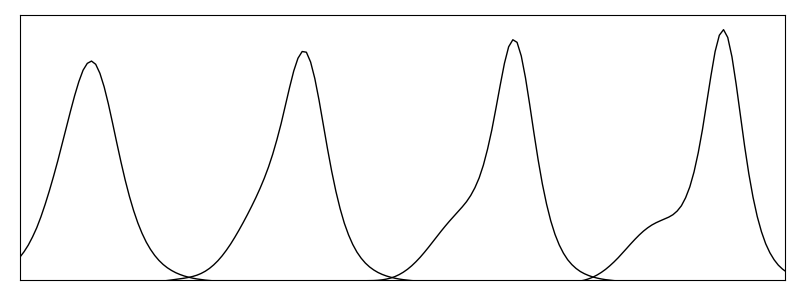
\includegraphics[width=.9\textwidth]{img/boussinesq low dispersion.png}
    \caption{Amplitude dispersion}
    \label{ampl_dispersion}
\end{subfigure}
\begin{subfigure}{\textwidth}
    \centering
    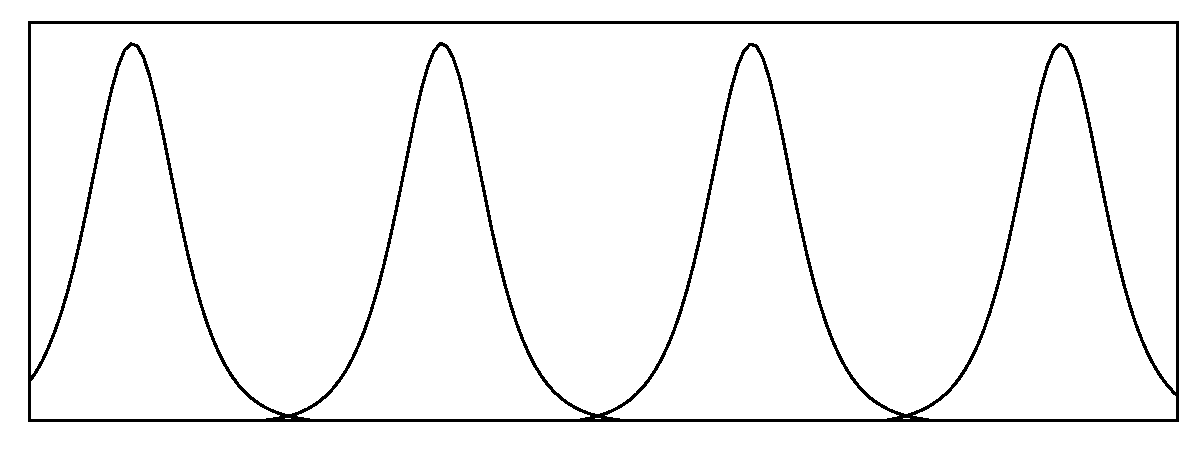
\includegraphics[width=.9\textwidth]{img/boussinesq.pdf}
    \caption{Frequency dispersion}
    \label{freq_dispersion}
\end{subfigure}
\end{figure}

In practice, this phenomenon does not happen. From linear wave theroy we know that the celerity depends not only on the water depth, but also on the wavenumber $k=2\pi/\lambda$. This is known as frequency dispersion and this mechanism is missing on the Saint-Venant equations. The introduction of some extra tems leads to the Boussinesq equations, which model the frequency dispersion. Once the frequency dispersio is included, classical soliton waves can be obtained. In a soliton wave, breaking never occurs during the propagation, since the non linear terms are in equilibrium with dispersive terms.


\subsubsection{Derivation of the modified Boussinesq equations}

There are different ways to derive the Boussinesq equations with slightly different results. Nwogu presented a general framework in \cite{nwogu1993}. A three dimensional wave field with free surface elevation $\eta(x_1, x_2, t)$ and water depth at rest $H(x_1, x_2)$ is considered. The fluid is governed by the Navier-Stokes equations but the shallow water asumptions are modified. The fluid is assumed to be incompressible and the flow is assumed to be irrotational. As in the shallow water equations, the vertical velocity is considered to be small, but the vertical acceleration is not negligible. The nonlinearity and dispersion ratios (\ref{nonlin_disp_ratios}) are assumed to be small. The last difference between the shallow water equations and the Boussinesq consist in considering the horizontal velocity at a specified water depth instead of the mean value.

\begin{figure}
    \centering
    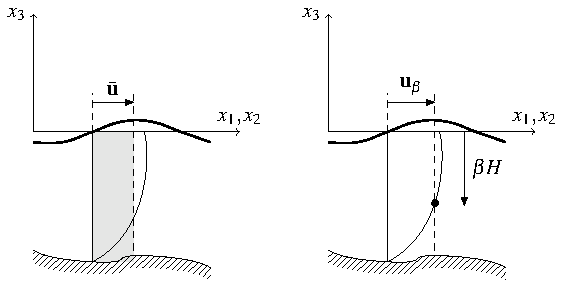
\includegraphics[width=.9\textwidth]{img/velocity_beta.pdf}
    \caption{The modified Boussinesq equations consider the velocity at an arbitrary depth $\beta H$ instead of the mean velocity}
\end{figure}

Finally, the fluid at the free surface has to satisfy a dynamic and kynematic bondary conditions. At the bottom, the fluid has to satysfy a kynematic boundary condition.

\begin{equation}\label{dyn_kyn_bc}
\begin{split}
p &= 0 \ , \quad \text{at } x_3=\eta \\
u_3 &= \pder{\eta}{t} + u_1 \pder{\eta}{x_1}  + u_2 \pder{\eta}{x_2} \ , \quad \text{at } x_3=\eta \\
u_3 &= -u_1 \pder{H}{x_1} -u_2 \pder{H}{x_2} \ , \quad \text{at } x_3=-H
\end{split}
\end{equation}

Then, the continuity and momentum equations are integrated from the bottom to the free surface and applying the boundary conditions (\ref{dyn_kyn_bc}). Since the averge horizontal velocity has been substituted by the velocity at a certatin depth, the vertical profile of the velocities must be known. The key of the Boussinesq equations consist in finding an assumption which preserves the the effect of the frequency dispersion. The horizontal velocities $\mathbb{u}=(u_1, u_2)$ are expanded in Taylor series from the seabed ($x_3=-H$),
\begin{multline} \label{seabed_taylor_expansion}
    \mathbf{u}(x_1,x_2,x_3,t) = \mathbf{u}(x_1,x_2,-H,t) + (z+H)\mathbf{u}_3(x_1,x_2,-H,t) \\ + \sfrac{1}{2}(z+H)^2\mathbf{u}_{3,3}(x_1,x_2,-H,t) + \dots
\end{multline}
where the $3$ subscript denotes differenctiation with respecct to $x_3$.
Finally, the equations are evaluated at an arbitrary depth $x_3=\beta H$ and the set of Boussinesq-type equations are:

\begin{subequations} \label{bsq_eq}
\begin{equation} \label{bsq_eq_mass}
    \pder{\eta}{t} + \nabla \cdot \left((H+\eta)\mathbf{u}_\beta\right) + \nabla \cdot \mathbf{J}_\eta = 0
\end{equation}
\begin{equation} \label{bsq_eq_mom}
    \pder{\mathbf{u}_\beta}{t} + \nabla \eta + (\mathbf{u}_\beta \cdot \nabla) \mathbf{u}_\beta + \mathbf{J}_u = \mathbf{0}
\end{equation}
\end{subequations}
where the auxiliary fields $\mathbf{J}_\eta$ and $\mathbf{J}_u$ introduce the dispersive mechanism and are defined according to the following expressions
\begin{subequations}
\begin{equation}
    {J}_\eta =
        C_1 H^3 \nabla \nabla \cdot \mathbf{u}_\beta +
        C_3 H^2 \nabla \nabla \cdot (H \mathbf{u}_\beta) 
\end{equation}
\begin{equation}
    {J}_u =
        C_2 H^3 \nabla \nabla \cdot \pder{\mathbf{u}_\beta}{t} +
        C_4 H^2 \nabla \nabla \cdot \pder{(H \mathbf{u}_\beta)}{t} 
\end{equation}
\end{subequations}
and the $C_i$ constants depend on the choice of $\beta$
\begin{equation}
    C_1=\frac{1}{2}\left(\beta^2-\frac{1}{3}\right)\ ,
    C_2=\frac{\beta^2}{2}\ ,
    C_3=\beta + \frac{1}{2}\ ,
    C_4=\beta
\end{equation}


\subsubsection{Linear dispersion properties and range of applicability}

This equations present as a free parameter $\beta$ the relative elevation at which the velocity is evaluated. Its value goes from $-1$ at the seabed, to $0$ at the free surface. Since the equations are an approximation of the fully dispersive and nonlinear problem, the parameter $\beta$ is choosen to minimize the errors introduced by the approximation.
In fact, the original Boussinesq equations does no present any dispersive term in the mass balance equation (\ref{bsq_eq_mass}) and correspond to a specific choice of $\beta$.

The parameter $\beta$ is fixed to $-0.531$ in \cite{nwogu1993}. This value has been obtained reducing the equations (\ref{bsq_eq}) to one dimension and flat bottom. Then, a trial function of small amplitude periodic wave of the type
\begin{equation*}
    \eta = a_0 \exp(i(kx-\omega t)) \ , \quad u_\beta = u_0 \exp(i(kx-\omega t))
\end{equation*}
is substitured into (\ref{bsq_eq_mass}) and (\ref{bsq_eq_mom}). After some algebraic manipulation the following expression for the phse speed is obtained:
\begin{equation}
c^2 = \frac{\omega^2}{k^2} = gh
    \left(\frac{
        1-\left(\frac{1}{2}\beta^2 + \beta + \frac{1}{3}\right)(kh)^2
    }{
        1-\left(\frac{1}{2}\beta^2 + \beta\right)(kh)^2
    }\right)
\end{equation}
The relation between the frequency and the wavelength is also known as \emph{dispersion relation}.
By the other hand, the dispersion relation given by the Linear wave theory or Airy theory is given by
\begin{equation}
c^2 = gh \frac{\tanh kh}{kh}
\end{equation}

Finally, the value of $\beta$ has been chosen to minimize the error at the range of applicability. Some other classical values of beta were obtained in \cite{madsen1991,murray1989}. Figure \ref{phase_speed_beta} shows the sensitivity of the phase speed depending on the parametesr $\beta$. The shallow water equations, which drop the dispersinve terms of equations (\ref{bsq_eq}) are only valid for the shallow water regime ($kh<0.3$). Fixing the free parameter $\beta=-0.531$ extend the range of applicability of the Boussinesq equations to intermediate depths ($kh<3$).

\begin{figure}
    \centering
    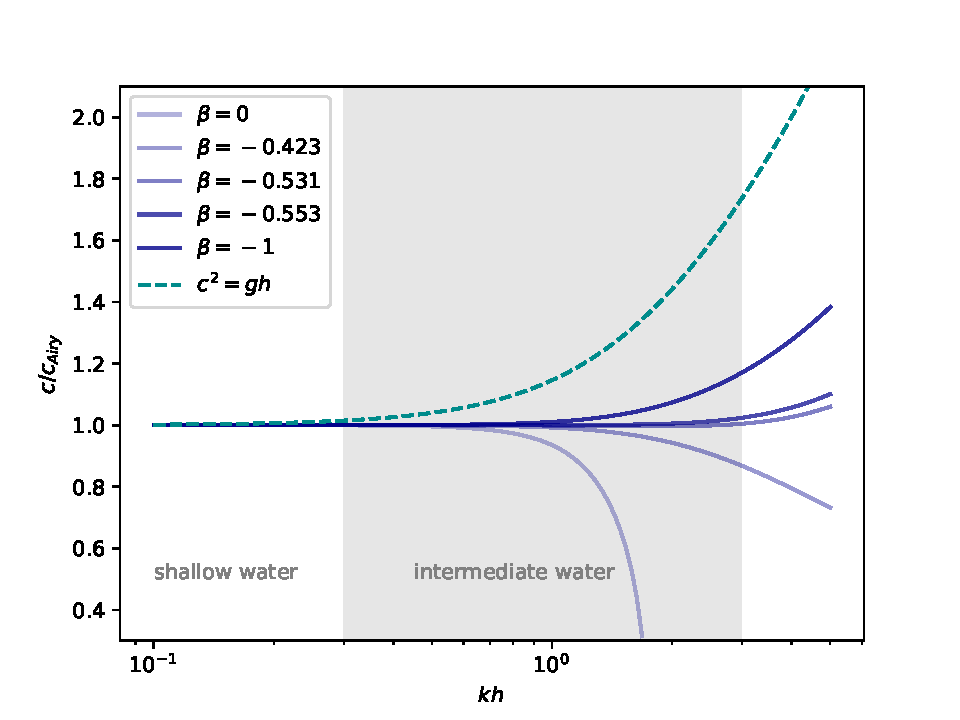
\includegraphics[width=.8\textwidth]{img/dispersion_beta.pdf}
    \caption{Comparison of normalized phase speeds for different values of $\beta$}
    \label{phase_speed_beta}
\end{figure}

According to \cite{ursell1953} the nonlinearity and dispersion parameters $\epsilon$ and $\mu$ can be used for an alternative classification:

\begin{description}
    \item[$\epsilon \ll \mu$]  This configuration correspond to the case where frequency dispersion dominates the problem and linear or Airy theory must be used.
    \item[$\epsilon \sim \mu$] In this case frequency and amplitude dispersion are of the same magnitude and the Boussinesq approximation can be used.
    \item[$\epsilon \gg \mu$] In this situation the amplitude dispersion dominates the problem and the wave will eventually break. This can be simulated using the Saint-Venant or shallow water equations. Since the vertical velocityis assumed negligible, the pressure distribution is assumed to be constant.
\end{description}






\subsubsection{Condiciones de contorno absorbentes}

Es frecuente que que sea necesario acotar el dominio de estudio, imponiendo condiciones abiertas. Estas condiciones de contorno abiertas o radiantes han de permitir la salida de ondas, al mismo tiempo que garantizan la consistencia matemática del sistema de ecuaciones. Al mismo tiempo que la expresión matemática ha de garantizar la existencia de la solución, tambień ha de ser compatible con la disretización numérica empleada para el interior del dominio. Generalmente, se denomina condiciones de contorno radiantes a la formulación analítica y condiciones de contorno absorbentes al método numerico \cite{navon2004}.
Se busca un equilibrio entre la precisión con la que se aproxima la condición de radiación (reducción de reflexión) y el coste computacional.

En este sentido, es de gran importancia que el método numérico junto con las condiciones escogidas, resulten en un esquema estable, al mismo tiempo que las oscilaciones espúreas generadas por la reflexión sean pequeñas.
Por otro lado, hay que asegurar que el cálculo de las condiciones de contorno no concluyan en un coste computacional excesivo comparado con el del dominio interior.

La primera consideración es que, tomando $\eta$ como la superficie libre y en un caso unidireccional, una función de onda presentará una condición radiante donde verifique que
\begin{equation} \label{radiation_condition}
    \pder{\eta}{t} + c \cos(\theta)\pder{\eta}{x} = 0
\end{equation}
donde $\eta$ es la variación de la superficie libre, expresada en términos del calado $h$ y la topografía $z_b$, $c$ es la velocidad de propagación de las ondas y $\theta$ es el ángulo con la frontera.

Algunos autores como Engquist propusieron aproximaciones locales altamente disipativas \cite{engquist1977}, más adelante Bayliss \cite{bayliss1982} exploró las condiciones radiantes para las ecuaciones de Helmholtz. De modo similar, Collino \cite{collino1993} extendió la formulación empleando derivadas de mayor orden. Sin embargo, la generalización para las ecuaciones de Euler o, análogamente, a las ecuaciones de aguas poco profundas en 2D no es trivial. Por un lado, el ángulo de incidencia $\theta$ no es conocido \emph{a priori}, dando lugar a la reflexión de la componente no alineada. Por otro lado, las ecuaciones de aguas poco profundas son disperivas y no hay una sola celeridad que caracterice el sistema \cite{wei1995}. Es decir, hay tres ondas superpuestas que se propagan con velocidades diferentes. Por ejemplo, se pueden reescribir las ecuaciones \ref{general_sw} en variables características, mediante la diagonalización de la matrices tangentes $\mathbf{A}_i$ de la forma
\begin{equation}
    \pder{\bm\Phi_j}{t} + \bm\Lambda_i \pder{\bm\Phi_j}{x_i} = 0
\end{equation}
donde $\bm\Lambda$ es una matriz diagonal tal que $\bm A_i = \bm T_i \bm\Lambda_i \bm T_i^{-1}$. El problema resultante es la conveción de tres ondas, cada una asociada a las velocidades $\lambda_i$, que corresponden a $u-c$, $u$ y $u+c$. Los distintos valores de $\lambda_i$ determinan si cada condición de contorno se trata de una entrada o salida, y si es sub-crítica o super-crítica.

A parte de tener que imponer la condición radiante para las tres ondas, la validez de este método es limitada, ya que en más de 1D no existe una formulación genuina basada en caracterísitcas. Puede encontrarse un desarrollo completo en \cite{lie2001}.

Muchas de las aproximaciones propuestas \cite{israeli1981,navon2004,carmigniani2018} consisten en relajar la condición (\ref{radiation_condition}) añadiendo un término disipador $K$
\begin{equation} \label{radiation_absorbing_condition}
    \pder{\eta}{t} + c \cos(\theta)\pder{\eta}{x} = -K\eta
\end{equation}
y extendiendo el dominio en una distancia $d$. Esta aproximación se suele emplear en combinación con condiciones absorbentes locales \cite{wei1995}.

Otra de las vías exploradas es la Perfectly Matched Layer (PML) \cite{berenger1994}, que ha sido ampliamente utilizada en la literatura. Presenta el inconveniente de tener que imponer tratamietos especiales en las esquinas.

Posteriormente, esta metodología fue empleada en combinación con las fronteras absorbentes de alto orden, dando lugar a la Double Absorbing Boundary (DAB), propuestas por Hagstrom y Rabinovich \cite{hagstrom2014,rabinovich2015}. Esta úlima metodología ubica dos fronteras paralelas, separadas por una pequeña distancia. Presenta la ventaja de no tener que incorporar derivadas en la dirección normal ni tener que aplicar tratamientos especiales a las esquinas.

Dada la simplicidad de la formulación, se ha optado por introducir solamente una capa de esponja, sigiendo las formulaciones de \cite{israeli1981} y \cite{carmigniani2018}. Se ha introducido un factor disipador Newtoniano de la siguiente forma análogo a la fricción de fondo $S_f$ de la siguiente forma:
\begin{equation}
    S_a = -\gamma(\mathbf{x}) \mathbf{u}
\end{equation}


El término disipador $\mathbf{\gamma}$ varía desde cero hasta al valor máximo $\gamma_{\max}$ junto a la frontera. Sigue un ley exponencial \cite{peric2018} que depende del exponente $n$. Los parámetros del grosor de la esponja $d_0$ y valor máximo deben determinarse para casa caso, según la longitud de onda de las olas.

\begin{equation} \label{exponential_sponge_layer}
    \gamma(\mathbf{x}) = \gamma_{\max} \mathcal{H}(d_0 - d(\mathbf{x})) \frac{e^{\left(\frac{d_0 - d(\mathbf{x})}{d_0}\right)^n} - 1}{e - 1}
\end{equation}
where $\mathcal{H}$ is the Heaviside function, $d$ is the distance from a point to the computational boundary.

En la figura \ref{absorbing_boundary} se muestra la propagación de un tren de olas mono-cromáticas. En un extremo del dominio se generan las olas, en el extremo opuesto hay una frontera absorbente. Estudios como el realizado por \cite{carmigniani2018} muestran que diversos valores de absorción, grosor de la esponja, o de la función exponencial (\ref{exponential_sponge_layer}) pueden provocar reflexiones no deseadas. Por ejemplo, una excesiva absorción provocaría una reflexión al inicio de la capa de esponja.

Se ha elegido $n=3$ para la expresión (\ref{exponential_sponge_layer}), por ser un valor que minimiza considerablemente la reflexión (ver \cite{carmigniani2018}). Queda hacer un análisis de sensibilidad de los parámetros $d_0$ y $\gamma_{\max}$.

Resulta práctico expresarlos en términos relativos a la longitud de onda $\lambda$ y a la frecuencia $\omega$. En la práctica, el grosor de la capa esponja suele ser $d_0 \approx 2\lambda$ y el coefficiente de absorción $\gamma \approx 0.5\omega$. Mientras que el coeficiente de reflexión es monótono decreciente con grosor de la capa, presenta un mínimo local respecto a la frecuencia. Esto hace que para un tren de olas sea recomendable ajustar los parámetros de acuerdo con la máxima longitud de onda.


\begin{figure}
    \centering
    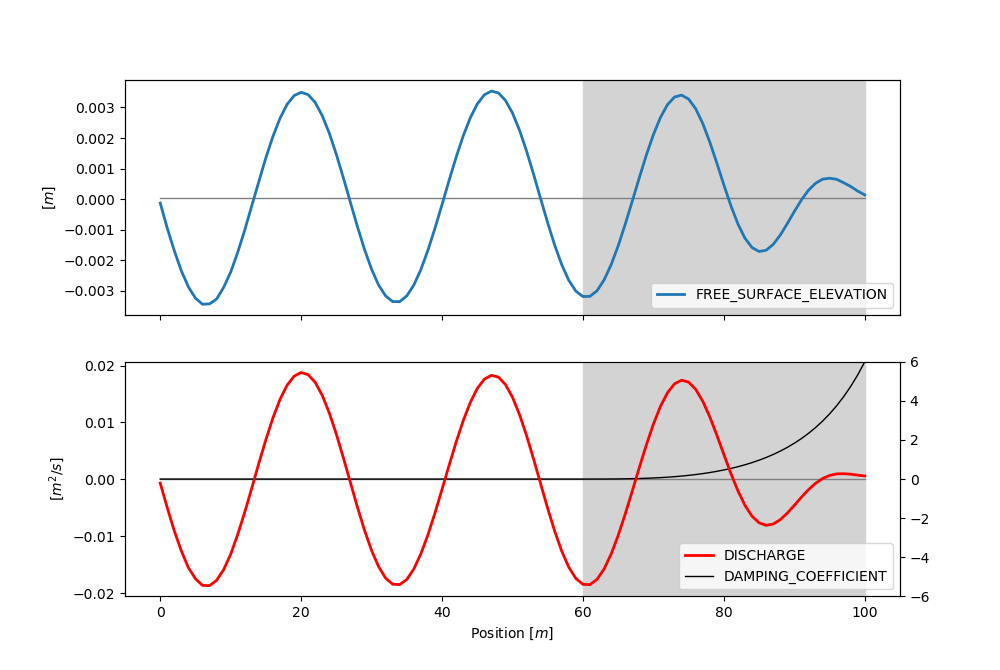
\includegraphics[width=.8\textwidth]{img/absorbing_boundary.png}
    \caption{Propagación y absorción de un tren de olas. La región sombreada de gris muestra el grosor de la capa esponja.}
    \label{absorbing_boundary}
\end{figure}




